\section{Taylor公式与局部近似}
\label{sec:ru-taylor}
\label{sec:analysis-taylor-approximation}

一次近似$f(a)+f'(a)h$只用到函数值和斜率，误差是$o(h)$。要提高精度，可以让近似多项式在$a$处与$f$有更多阶相同的导数。
本节先说明这样的多项式怎样确定、误差怎样控制，再把它用于指数函数和三角函数，得到它们的级数展开与Euler公式，最后用同样的工具分析差分近似的误差。

\subsection{Taylor多项式及余项}
\label{sec:ru-taylor-remainders}

设$p(x)=\sum_{k=0}^nc_k(x-a)^k$。逐次求导并代入$x=a$，除了第$k$项外的各项都变为零，得到$p^{(k)}(a)=k!\,c_k$。
所以，要让$p$在$a$处与$f$的前$n$阶导数都相同，系数只能取$c_k=f^{(k)}(a)/k!$。称
\[
 T_n(a+h)=\sum_{k=0}^n\frac{f^{(k)}(a)}{k!}h^k
\]
为$f$在$a$处的$n$阶\term{Taylor多项式}（Taylor polynomial），阶乘来自对$h^k$求$k$次导数。$n=1$时它就是一次近似。
截去的部分$R_n(h)=f(a+h)-T_n(a+h)$称为余项，把函数写成Taylor多项式加余项的等式称为\term{Taylor公式}（Taylor formula）。首先关心的是$h\to0$时余项的阶。
\begin{theorem}[带Peano余项的Taylor公式]
\label{thm:ru-taylor-peano}
设$n\geq1$，$f$在$a$的某个邻域内$n-1$阶可导，且$f^{(n)}(a)$存在，则$h\to0$时
\[
 f(a+h)=\sum_{k=0}^n\frac{f^{(k)}(a)}{k!}h^k+o(h^n).
\]
\end{theorem}
\begin{proof}
对$n$归纳。$n=1$就是可微的定义~\eqref{eq:analysis-scalar-first-order}。设结论对$n-1$成立。$R_n$在$h=0$处为零，它关于$h$的导数$R_n'(h)=f'(a+h)-\sum_{k=1}^n\frac{f^{(k)}(a)}{(k-1)!}h^{k-1}$
恰是$f'$在$a$处的$n-1$阶余项，由归纳假设为$o(h^{n-1})$。由中值定理，$R_n(h)=R_n(h)-R_n(0)=R_n'(\xi)h$，$\xi$在$0$与$h$之间，于是$|R_n(h)|\leq\sup_{|t|\leq|h|}|R_n'(t)|\cdot|h|=o(h^n)$。
\end{proof}
Peano余项只说明误差的阶，不给出指定$h$处的误差大小。若函数在整段上有更高阶的导数，可以把余项写成某个中间点处的导数。
\begin{theorem}[带Lagrange余项的Taylor公式]
\label{thm:analysis-taylor-lagrange}
设$n\geq0$，$h\neq0$，$f$在包含$a$与$a+h$之间闭线段的某个开区间上$n+1$阶可导，则存在严格位于$a$与$a+h$之间的$\xi$，使
\begin{equation}
 f(a+h)=\sum_{k=0}^n\frac{f^{(k)}(a)}{k!}h^k+\frac{f^{(n+1)}(\xi)}{(n+1)!}h^{n+1}.
 \label{eq:analysis-taylor-arbitrary-order}
\end{equation}
若该线段上$|f^{(n+1)}|\leq M$，则$|R_n(h)|\leq M|h|^{n+1}/(n+1)!$。
\end{theorem}
\begin{proof}
记$T(t)=\sum_{k=0}^nf^{(k)}(a)(t-a)^k/k!$，$R=f(a+h)-T(a+h)$，令$H(t)=f(t)-T(t)-R\,(t-a)^{n+1}/h^{n+1}$。
则$H(a+h)=0$，且$H(a)=H'(a)=\cdots=H^{(n)}(a)=0$。先在$a$与$a+h$之间对$H$用Rolle定理得$\xi_1$使$H'(\xi_1)=0$；再在$a$与$\xi_1$之间对$H'$用Rolle定理得$\xi_2$，如此继续。
共用$n+1$次后得到严格位于$a$与$a+h$之间的$\xi$，使$H^{(n+1)}(\xi)=0$。由$T^{(n+1)}=0$，这就是$f^{(n+1)}(\xi)-(n+1)!\,R/h^{n+1}=0$。
\end{proof}
$n=0$时公式就是Lagrange中值定理。误差界说明近似的精度同时取决于阶数、步长和高阶导数的界，三者都可以具体计算。
例如$f(x)=x^3-3x$在$a=1/2$处的二阶Taylor多项式为$T_2=-\tfrac{11}8-\tfrac94h+\tfrac32h^2$，由$f'''\equiv6$，余项恰为$h^3$；取$h=0.1$，$T_2$与真值$-1.584$相差$0.001$。
余项的第三种写法是积分形式，它不含未知的中间点，需要积分，留到第~\ref{sec:ru-integration-by-parts}节推导。

有限阶展开、Taylor级数与“函数等于自身的Taylor级数”是三件不同的事。若$f$无穷次可微，可以写出无穷级数$\sum_kf^{(k)}(a)(x-a)^k/k!$，称为$f$在$a$处的Taylor级数；
但这个级数未必收敛到$f$。下面的例子中，Taylor级数在整条实轴上收敛，却只在一点等于原函数。
\begin{example}[光滑但不等于自身Taylor级数的函数]
\label{ex:ru-smooth-not-analytic}
令$f(0)=0$，$x\neq0$时$f(x)=e^{-1/x^2}$。对$x\neq0$归纳可知$f^{(k)}(x)=P_k(1/x)e^{-1/x^2}$，其中$P_k$是多项式。
由$e^u\geq u^m/m!$（$u>0$）取$u=1/x^2$，得$|x|^{-j}e^{-1/x^2}\leq m!\,|x|^{2m-j}$，取$2m>j$即知它在$x\to0$时趋于零。
再在原点用差商逐阶验证，可得$f^{(k)}(0)=0$对每个$k$成立。于是$f$的Taylor级数恒为零，而$x\neq0$时$f(x)>0$。
\end{example}
所以无穷次可微还不足以保证函数能由Taylor级数表示。对具体函数，必须另外证明余项趋于零；下面对指数和三角函数完成这一步。

\subsection{指数函数的展开}
\label{sec:ru-exp-expansion}

由$(e^x)'=e^x$，指数函数在$0$处的各阶导数都是$1$，Taylor系数为$1/k!$。由Lagrange余项，对固定的$x$，
\[
 \Bigl|e^x-\sum_{k=0}^n\frac{x^k}{k!}\Bigr|=\frac{e^\xi|x|^{n+1}}{(n+1)!}\leq\frac{e^{|x|}|x|^{n+1}}{(n+1)!},
\]
$\xi$在$0$与$x$之间。右侧是收敛级数$\sum|x|^k/k!$的项，趋于零，所以余项趋于零，$e^x=\sum_{k\geq0}x^k/k!$。
这与第~\ref{sec:ru-elementary-limits}节用级数定义的指数一致。那里级数是定义，这里则是从导数出发，用余项估计证明函数等于级数，两条路线得到同一个对象。

余项估计还说明了截断要取多少项。在区间$[-A,A]$上，误差不超过$e^AA^{n+1}/(n+1)!$，这个界对整个区间统一成立。
例如$A=1$、$n=7$时误差不超过$e/8!\approx6.7\times10^{-5}$；区间越大，所需阶数越高。一般底数的指数$a^x=e^{x\log a}$可以把$x\log a$代入上式处理。

\subsection{三角函数的展开与复指数}
\label{sec:ru-trig-expansion-complex-exponential}

正弦和余弦的各阶导数按四步循环，在$0$处的值依次为$\sin$：$0,1,0,-1,\ldots$，$\cos$：$1,0,-1,0,\ldots$。各阶导数的绝对值都不超过$1$，Lagrange余项满足$|R_n(x)|\leq|x|^{n+1}/(n+1)!\to0$，所以
\[
 \sin x=\sum_{k=0}^\infty\frac{(-1)^kx^{2k+1}}{(2k+1)!},\qquad\cos x=\sum_{k=0}^\infty\frac{(-1)^kx^{2k}}{(2k)!},
\]
对所有实数$x$成立。截断误差也可以直接读出：$\sin x\approx x-x^3/6$的四次项为零，用$n=4$的余项得误差不超过$|x|^5/120$；$x=0.5$时约为$2.6\times10^{-4}$。

这两个级数与指数级数只差符号的排列，提示三者有联系。为看清这一点，需要让指数级数接受复数输入。
复数列$z_n\to z$定义为$|z_n-z|\to0$；由$|\operatorname{Re}w|,|\operatorname{Im}w|\leq|w|\leq|\operatorname{Re}w|+|\operatorname{Im}w|$，它等价于实部、虚部分别收敛。
若$\sum|z_k|<\infty$，则实部级数与虚部级数都绝对收敛，因而$\sum z_k$收敛，绝对收敛的结论由此搬到复数。
对每个复数$z$，$\sum|z|^k/k!=e^{|z|}$有限，所以可以定义复指数
\[
 e^z=\sum_{k=0}^\infty\frac{z^k}{k!}.
\]
取纯虚输入$z=i\theta$。由$i^2=-1$，$i^k$按$1,i,-1,-i$循环，部分和$S_{2N+1}$的偶次项全为实数、奇次项全为虚数：
\[
 S_{2N+1}(i\theta)=\sum_{k=0}^N\frac{(-1)^k\theta^{2k}}{(2k)!}+i\sum_{k=0}^N\frac{(-1)^k\theta^{2k+1}}{(2k+1)!}.
\]
令$N\to\infty$，实部与虚部分别趋于刚证明的余弦与正弦展开；整个级数收敛，它的和等于这个子列的极限。于是得到\term{Euler公式}（Euler's formula）
\[
 e^{i\theta}=\cos\theta+i\sin\theta.
\]
这里只把偶次项与奇次项分开读出，没有改变求和次序。

回到复数的三角形式$z=r(\cos\theta+i\sin\theta)$，Euler公式把它写成指数形式$z=re^{i\theta}$：$r$是模，$\theta$是辐角。
第~\ref{sec:ru-complex-geometry}节的“模相乘、辐角相加”变为$r_1e^{i\theta_1}\cdot r_2e^{i\theta_2}=r_1r_2e^{i(\theta_1+\theta_2)}$，整数次幂变为$(re^{i\theta})^n=r^ne^{in\theta}$，三角形式与指数形式由此统一。
特别地，$e^{i\pi}=-1$，$e^{2\pi i}=1$，辐角相差$2\pi$的整数倍正对应$e^{i\theta}$的周期性。本书只使用复数级数，不展开复变函数的微积分。

\subsection{差分近似和步长选择}
\label{sec:ru-finite-differences}

只能计算函数值时，常用差商近似导数。Taylor公式可以说明这种近似的误差有多大。设$f$在$x$附近足够光滑，前向差分的误差由二阶Taylor公式得到：
\[
 \frac{f(x+h)-f(x)}h=f'(x)+\frac{f''(\xi)}2h,
\]
所以$|f''|\leq M_2$时截断误差不超过$M_2h/2$，与$h$同阶。中心差分对称地取两侧，把$f(x\pm h)$各展开到三阶后相减，偶次项抵消：
\[
 \frac{f(x+h)-f(x-h)}{2h}=f'(x)+\frac{f'''(\xi_1)+f'''(\xi_2)}{12}h^2,
\]
$|f'''|\leq M_3$时误差不超过$M_3h^2/6$，与$h^2$同阶，代价是需要三阶导数的界。
用$f(x)=e^x$在$x=0$处核对：取$h=0.1$，前向差分为$(e^{0.1}-1)/0.1\approx1.0517$，误差约$0.052$，接近$h/2=0.05$；中心差分为$(e^{0.1}-e^{-0.1})/0.2\approx1.00167$，误差约$0.00167$，接近$h^2/6\approx0.00167$。

上面的误差分析假定函数值是精确的。实际计算中，函数值本身带有数据误差或舍入误差。设算得的值$\tilde f$满足$|\tilde f-f|\leq\eta$，前向差分的总误差就不超过
\[
 \frac{M_2h}2+\frac{2\eta}h.
\]
第一项是截断误差，随$h$减小而减小；第二项是函数值误差，被除以$h$后放大，随$h$减小而增大。两者之和在$h=2\sqrt{\eta/M_2}$处最小，最小值为$2\sqrt{M_2\eta}$。
以双精度浮点计算为例，$\eta$约为$10^{-16}$乘以函数值的大小，前向差分的合适步长约为$10^{-8}$，而不是越小越好；中心差分的总误差为$M_3h^2/6+\eta/h$，合适步长约为$10^{-5}$\scite{math-nocedal2006numerical}。
图~\ref{fig:ru-finite-difference-error}画出了实际计算的误差：步长大于最优值时，误差沿截断误差的斜率下降；小于最优值后，舍入误差占主导，误差反而上升并剧烈波动。
这里只讨论误差的来源与竞争，系统的数值分析不在本书范围之内。

\begin{figure}[!htbp]
 \centering
 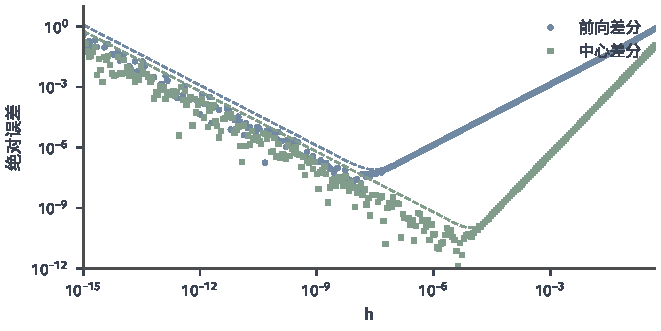
\includegraphics[width=112mm]{figures/01-mathematical-preliminaries-upper/02-real-numbers-and-univariate-functions/matplotlib/finite-difference-error/figure.pdf}
 \caption{用双精度浮点数计算$f(x)=e^x$在$x=1$处导数的差分误差，横轴为步长$h$，两轴均为对数刻度。蓝点为前向差分，绿点为中心差分；虚线是误差模型$eh/2+2\epsilon_{\mathrm{m}}e/h$与$eh^2/6+\epsilon_{\mathrm{m}}e/h$，$\epsilon_{\mathrm{m}}\approx2.2\times10^{-16}$为机器精度。大步长段的斜率分别为$1$与$2$，小步长段的误差随$h$减小而增大。}
 \label{fig:ru-finite-difference-error}
\end{figure}
